\documentclass[11pt]{article}

% ------------------------------------------------------------------ preamble
\usepackage[margin=1.1in]{geometry}
\usepackage{amsmath,amssymb}
\usepackage{booktabs}
\usepackage{graphicx}
\usepackage{microtype}
\usepackage{lmodern}
\usepackage[T1]{fontenc}
\usepackage{xcolor}
\usepackage{caption}
\usepackage{float}
\usepackage[hidelinks,colorlinks=true,linkcolor=blue!50!black,citecolor=blue!50!black,urlcolor=blue!50!black]{hyperref}

\captionsetup{font=small,labelfont=bf,width=0.92\linewidth}
\graphicspath{{../assets/}}

\newcommand{\fable}{Claude Fable~5}
\newcommand{\sol}{GPT-5.6}

\title{\textbf{No Detectable Difference: A Blocked Factorial Experiment\\
Comparing Claude Fable~5 and GPT-5.6\\
on Proven-Solvable Coding Tasks}}
\author{Drake Griffith\\
\small Actual Intelligence Labs\\
\small \texttt{christopherg@actualintelligencelabs.ai}}
\date{July 10, 2026}

\begin{document}
\maketitle

\begin{abstract}
\noindent
We report a controlled comparison of two frontier coding agents ---
\fable{} (Anthropic, via the \texttt{claude} CLI) and \sol{} ``Sol''
(OpenAI, via the \texttt{codex} CLI) --- across 154 runs of a full-factorial
designed experiment: model $\times$ reasoning effort $\times$ harness,
blocked by task, with replicated runs treated as Bernoulli trials and
seed-interleaved run order. All nine tasks were proven solvable before any
model ran. Both models passed every solo run (152/152); a per-cell perfect
score of $24/24$ carries a 95\% Wilson interval of $(0.862,\,1.000)$, and the
paired head-to-head McNemar test produced zero discordant pairs --- \emph{no
detectable difference}, which is a weaker and more honest claim than
``equal.'' Raising the reasoning-effort setting changed cost but not outcome:
pass rate was 100\% at every effort level while \sol{} at high effort spent
$\approx$80\% more output tokens than at low. An exact sign-flip permutation
test on per-task median $\log$(total tokens) shows \fable{} materially
cheaper per solved task ($p = 0.0039$), subject to a vendor-incomparability
caveat on input-token accounting. Transcripts were judged blind by two
independent model judges whose scores agreed within one point on 96\% of 139
dual-judged runs. The headline finding is a ceiling effect: the suite was
too easy to rank the models, and we say so rather than invent a winner. We
publish the full design, exact statistics, power analysis, and limitations,
and outline the harder-tier follow-up experiment.
\end{abstract}

% ---------------------------------------------------------------- section 1
\section{Introduction}

Most public comparisons of coding models are anecdotes: one person, one
prompt, two tools, and a preference. Because large-language-model inference
is non-deterministic, a single run measures what happened once, not what
happens on average --- and the average is the only quantity that matters
when choosing which tool a team ships with. Repeat the informal comparison
tomorrow and the ``winner'' can flip.

Structured public benchmarks have a complementary problem: frontier models
now cluster near the top of the standard suites, shrinking their power to
discriminate, and training-data contamination lets a model recall an answer
instead of reasoning to one. Jain et al.\ document both effects for code
generation and respond with a time-segmented benchmark of fresh contest
problems~\cite{jain2024livecodebench}.

We therefore ran a designed experiment rather than a leaderboard: identical
tasks and conditions, enough replication to separate signal from sampling
noise, exact small-sample statistics, and an explicit statement of what the
sample size can and cannot detect. The design follows standard
design-of-experiments practice (full factorial treatment structure, blocking,
randomization)~\cite{montgomery2017doe}.

Two results follow. First, a \emph{ceiling effect}: both models passed every
solo task, so this suite establishes that both clear the tier but cannot
rank them. Second, on this tier the reasoning-effort dial was pure cost:
identical outcomes at every setting, materially different token bills ---
consistent with the ``overthinking'' literature on efficient
reasoning~\cite{sui2025overthinking,su2025underthinking}.

% ---------------------------------------------------------------- section 2
\section{Experimental design}

\subsection{Treatment structure}

The run matrix is a full-factorial designed experiment:

\begin{itemize}
  \item \textbf{Factors.} Model (\fable{}, \sol{}) $\times$ reasoning effort
        (2--3 levels per model) $\times$ harness (bare CLI vs.\ a shared
        agent-instruction harness).
  \item \textbf{Blocking.} Task (eight T1/T2 tasks plus one T3 greenfield
        build). Every configuration sees every task, so task difficulty
        cancels out of all paired comparisons.
  \item \textbf{Replication.} $n=3$ repetitions per cell on T1/T2 tasks,
        $n=2$ on T3. Inference is non-deterministic; a single run is an
        anecdote, replicated runs estimate a pass \emph{rate}.
  \item \textbf{Randomization.} Run order is seed-interleaved (seed 1337) so
        time-of-day and API-load drift cannot systematically favor one model.
\end{itemize}

The experiment totals 154 official runs: a 120-run sweep~1 (bare, full
effort ladder), a sweep~2 adding harnessed conditions and the greenfield
build, and a small hybrid arm (Section~\ref{sec:hybrid}).

\subsection{Task suite}

Nine tasks, every one \emph{proven solvable before any model ran}:

\begin{itemize}
  \item \textbf{Four seeded-bug tasks} with deliberately subtle defects: an
        off-by-one in pagination, a naive-vs-timezone-aware datetime bug, a
        cache key that silently drops a dimension, and an async
        deduplication race.
  \item \textbf{Four feature tickets} written in a strict six-section ticket
        format.
  \item \textbf{One greenfield CLI build} (\texttt{splitcost}, a
        $\sim$200-line cost-splitting tool with a reference implementation).
\end{itemize}

Each task ships a self-test: the verifier fails on the broken starting code
and passes after the reference patch. All nine self-tests were green before
the experiment began, so any failure is attributable to the model, not to an
impossible task.

\subsection{Controlled conditions and blind dual judging}

Conditions were byte-identical across arms: the same harness instruction
files, the same prompts, and the same deterministic \texttt{verify.sh} gate
deciding pass/fail. Every transcript and diff was stripped of identifying
markers and scored blind by \emph{two} independent judges --- a Claude judge
and a GPT judge --- on a four-dimension rubric. Dual judging is a design
requirement, not decoration: LLM judges carry a documented self-preference
bias~\cite{wataoka2024selfpreference}, so a single-model judge grading its
own model's work is a conflict of interest built into the evaluator.
Judge agreement is reported as a result in its own right
(Section~\ref{sec:judges}).

% ---------------------------------------------------------------- section 3
\section{Outcome model}

Each run is a Bernoulli trial: pass (\texttt{verify.sh} exit 0) or fail. A
cell's empirical pass rate $\hat p = k/n$ estimates its Bernoulli parameter
$p$; within-cell scatter reflects the Bernoulli variance $p(1-p)$ plus model
non-determinism. All per-cell sample sizes are small ($n \in \{2,\dots,26\}$
per cell; $n=24$ per arm in the primary sweep-1 comparisons), so every test
in Section~\ref{sec:methods} is \emph{exact} --- no large-sample
approximation is used anywhere except the clearly labelled power search of
Section~\ref{sec:power}.

% ---------------------------------------------------------------- section 4
\section{Statistical methods}
\label{sec:methods}

All statistics are computed by a dependency-free reference implementation
(\texttt{runner/stats.py}, Python standard library only) directly from the
raw run and judgment logs; the implementation carries unit self-tests
against known values (Appendix~\ref{app:repro}).

\subsection{Wilson score intervals for per-cell pass rates}

For $k$ successes in $n$ trials with $z = z_{0.975} \approx 1.95996$, the
95\% Wilson score interval~\cite{wilson1927} is
%
\begin{equation}
\frac{\hat p + \dfrac{z^2}{2n}}{1 + \dfrac{z^2}{n}}
\;\pm\;
\frac{z}{1 + \dfrac{z^2}{n}}
\sqrt{\frac{\hat p (1-\hat p)}{n} + \frac{z^2}{4n^2}},
\qquad \hat p = \frac{k}{n}.
\label{eq:wilson}
\end{equation}
%
Unlike the naive Wald interval
$\hat p \pm z\sqrt{\hat p(1-\hat p)/n}$, the Wilson interval retains correct
coverage at small $n$ and at $\hat p \in \{0, 1\}$ --- exactly the regime of
this experiment, where cells post perfect scores. A perfect $24/24$ is
reported not as a bare ``100\%'' but with its interval $(0.862,\,1.000)$:
the data are consistent with a true failure rate anywhere from zero to
$\approx$14\%.

\subsection{McNemar's exact test for paired pass/fail comparisons}

Head-to-head comparisons pair runs by task $\times$ repetition, so task
difficulty cancels (the blocking pays off here). With $b$ pairs where arm A
passed and arm B failed, and $c$ pairs the other way, only the
$n_d = b + c$ \emph{discordant} pairs carry information about a difference.
The exact two-sided McNemar test~\cite{mcnemar1947} is a binomial test at
$\tfrac12$ on the discordant pairs:
%
\begin{equation}
p \;=\; \min\!\left(1,\;
2 \sum_{i=0}^{\min(b,c)} \binom{n_d}{i} \left(\tfrac{1}{2}\right)^{n_d}
\right).
\label{eq:mcnemar}
\end{equation}
%
When $n_d = 0$ the test is undefined and we report ``no evidence of
difference'' rather than a manufactured $p$-value.

\subsection{Exact sign-flip permutation test on token cost}

Token cost per solved task is compared with an exact paired permutation
test~\cite{fisher1935}. For each task $t$ we take the median of
$\log(\text{total tokens})$ over \emph{passing} runs for each model, form the
paired difference $d_t = \tilde m^{\text{Fable}}_t - \tilde m^{\text{Sol}}_t$,
and enumerate all $2^k$ sign assignments over the $k$ tasks:
%
\begin{equation}
p \;=\; \frac{\#\bigl\{ s \in \{-1,+1\}^k :
\bigl|\sum_{t} s_t\, d_t \bigr| \ge \bigl|\sum_{t} d_t\bigr| \bigr\}}{2^k}.
\label{eq:permutation}
\end{equation}
%
The log transform makes the statistic a ratio comparison and tames the
heavy right tail of token counts; medians over passing runs keep the
comparison per-solved-task.

\subsection{Power: the minimum detectable effect}
\label{sec:power}

The one deliberate approximation: the minimum detectable effect (MDE) is
found by a search over the normal-approximation power of a two-sided
two-proportion $z$-test. For per-arm size $n$, baseline $p_1$, alternative
$p_2 = p_1 + \delta$, and $\bar p = (p_1 + p_2)/2$,
%
\begin{equation}
\text{power}(\delta)
= \Phi\!\left(
\frac{\sqrt{n}\,\lvert\delta\rvert
      - z_{\alpha/2}\sqrt{2\,\bar p\,(1-\bar p)}}
     {\sqrt{p_1(1-p_1) + p_2(1-p_2)}}
\right),
\label{eq:power}
\end{equation}
%
and the MDE is the smallest $\delta$ with $\text{power}(\delta) \ge 0.80$ at
$\alpha = 0.05$. At $n = 24$ per arm and $p_1 = 0.5$ this gives
$\text{MDE} \approx 36.7$ percentage points. The reporting rule follows:
\emph{a gap smaller than the MDE gets a confidence interval, not a verdict}.
We say ``no detectable difference,'' never ``they're equal.''

% ---------------------------------------------------------------- section 5
\section{Results}

\subsection{Pass rates: both models hit the ceiling}

Sweep~1 was 120/120 across both models and every effort level; folding in
all solo sweep-2 runs gives \textbf{152/152} clean passes for every
configuration in which a model worked alone. Table~\ref{tab:wilson} reports
every cell with its Wilson interval (Eq.~\ref{eq:wilson});
Figure~\ref{fig:ceiling} draws the same intervals.

\begin{table}[H]
\centering
\small
\begin{tabular}{llllll}
\toprule
model & effort & harness & pass/$n$ & pass rate & 95\% Wilson CI \\
\midrule
Fable  & medium & bare    & 26/26 & 100\% & $(0.871,\,1.000)$ \\
Fable  & medium & harness & 14/14 & 100\% & $(0.785,\,1.000)$ \\
Fable  & high   & bare    & 24/24 & 100\% & $(0.862,\,1.000)$ \\
Hybrid & medium & harness & 2/2   & 100\% & $(0.342,\,1.000)$ \\
Sol    & low    & bare    & 26/26 & 100\% & $(0.871,\,1.000)$ \\
Sol    & low    & harness & 14/14 & 100\% & $(0.785,\,1.000)$ \\
Sol    & medium & bare    & 24/24 & 100\% & $(0.862,\,1.000)$ \\
Sol    & high   & bare    & 24/24 & 100\% & $(0.862,\,1.000)$ \\
\bottomrule
\end{tabular}
\caption{Per-cell pass rates with 95\% Wilson score intervals. Every cell is
perfect; the interval width is the honest small-$n$ uncertainty behind each
``100\%.'' (Hybrid: see the $2/4$ disclosure in Section~\ref{sec:hybrid}.)}
\label{tab:wilson}
\end{table}

\begin{figure}[H]
\centering
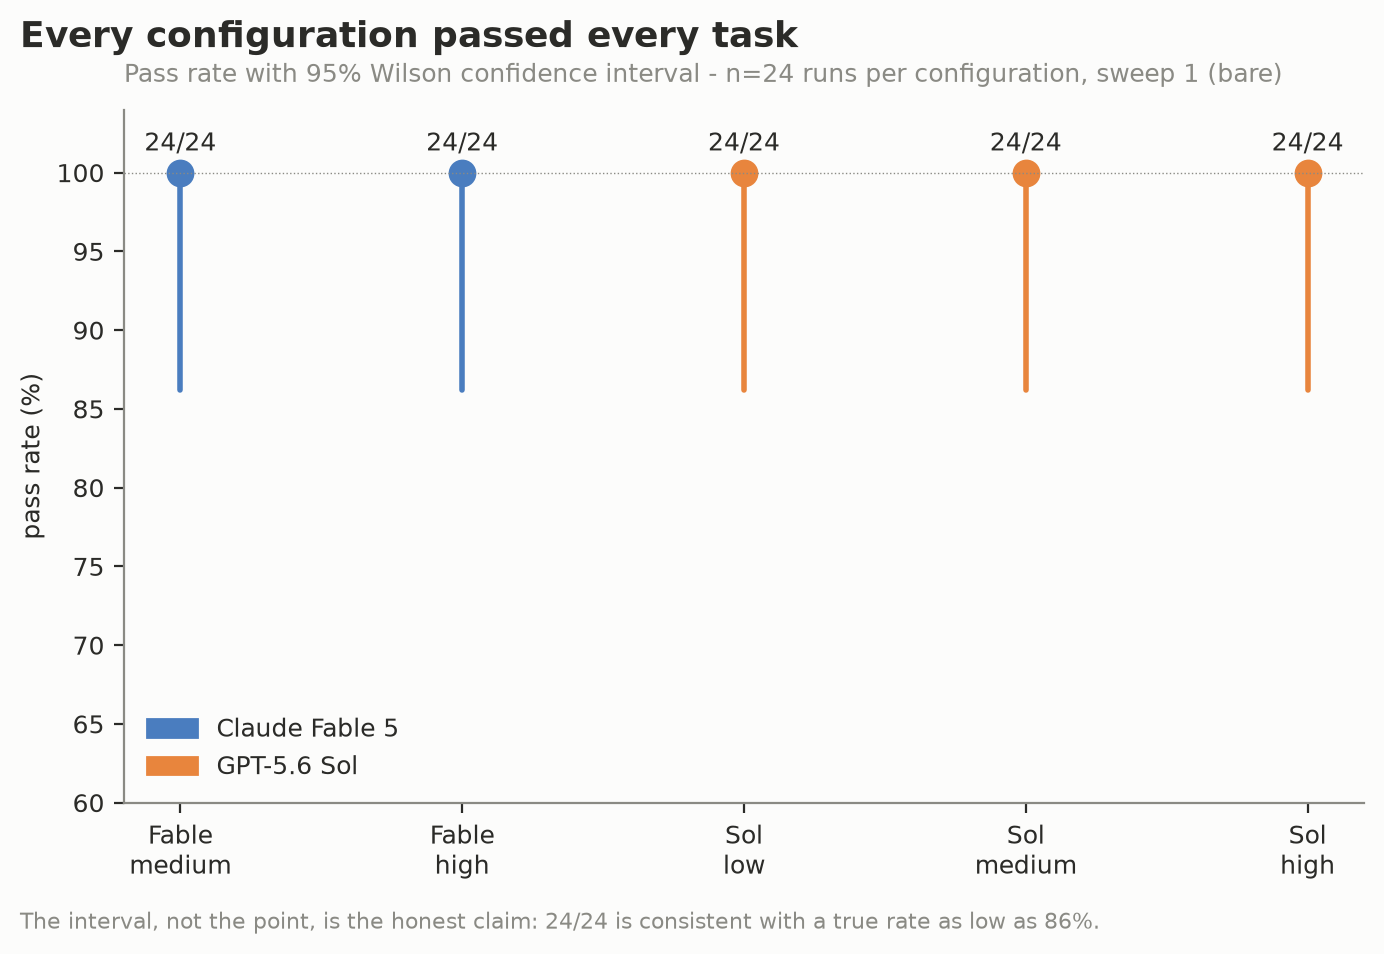
\includegraphics[width=0.9\linewidth]{1-pass-rate-ceiling.png}
\caption{Pass rate by configuration with 95\% Wilson intervals. Every bar
sits at 100\% with a lower bound set by the per-cell sample size --- perfect
scores drawn with their uncertainty.}
\label{fig:ceiling}
\end{figure}

\paragraph{Head-to-head.}
Each model's best effort was selected by pass rate with a
fewer-tokens tiebreak (Fable: medium; Sol: low), and the 26 task$\times$rep
pairs were compared with McNemar's exact test (Eq.~\ref{eq:mcnemar}). All 26
pairs were pass/pass: $b = c = 0$, zero discordant pairs, nothing to test.
Conclusion: \textbf{no detectable difference} between the models on this
suite --- a claim deliberately weaker than ``equal.''

\subsection{The effort dial bought nothing but tokens}

Pass rate was 100\% at every effort setting for both models, and every
adjacent-rung McNemar comparison (Fable high vs.\ medium; Sol medium vs.\
low, high vs.\ medium; 24 pairs each) had zero discordant pairs. What moved
was cost (Table~\ref{tab:sweep1}, Figure~\ref{fig:effort}): \fable{} at high
effort used $+16\%$ output tokens vs.\ medium (2{,}008 vs.\ 1{,}736 median);
\sol{} at high used $+80\%$ vs.\ low (1{,}966 vs.\ 1{,}095) and
$\approx 1.8\times$ the input tokens (174.7k vs.\ 95.2k). On tasks of this
tier, ``think harder'' settings are pure cost --- consistent with the
overthinking literature: reasoning models are poor at gauging problem
difficulty and elaborate on easy problems without improving
correctness~\cite{sui2025overthinking,su2025underthinking}.

\begin{table}[H]
\centering
\small
\begin{tabular}{lccccc}
\toprule
config & pass & output tok & input tok & wall clock & turns \\
\midrule
Fable / medium & 24/24 & 1{,}736 & 19{,}412  & 68.2\,s & 7 \\
Fable / high   & 24/24 & 2{,}008 & 19{,}398  & 58.8\,s & 6 \\
Sol / low      & 24/24 & 1{,}095 & 95{,}248  & 31.9\,s & 1 \\
Sol / medium   & 24/24 & 1{,}534 & 138{,}252 & 49.0\,s & 1 \\
Sol / high     & 24/24 & 1{,}966 & 174{,}662 & 63.7\,s & 1 \\
\bottomrule
\end{tabular}
\caption{Sweep-1 configurations (medians, $n=24$ per row). Input tokens are
CLI-reported and \emph{not comparable across vendors}
(Section~\ref{sec:inputtokens}).}
\label{tab:sweep1}
\end{table}

\begin{figure}[H]
\centering
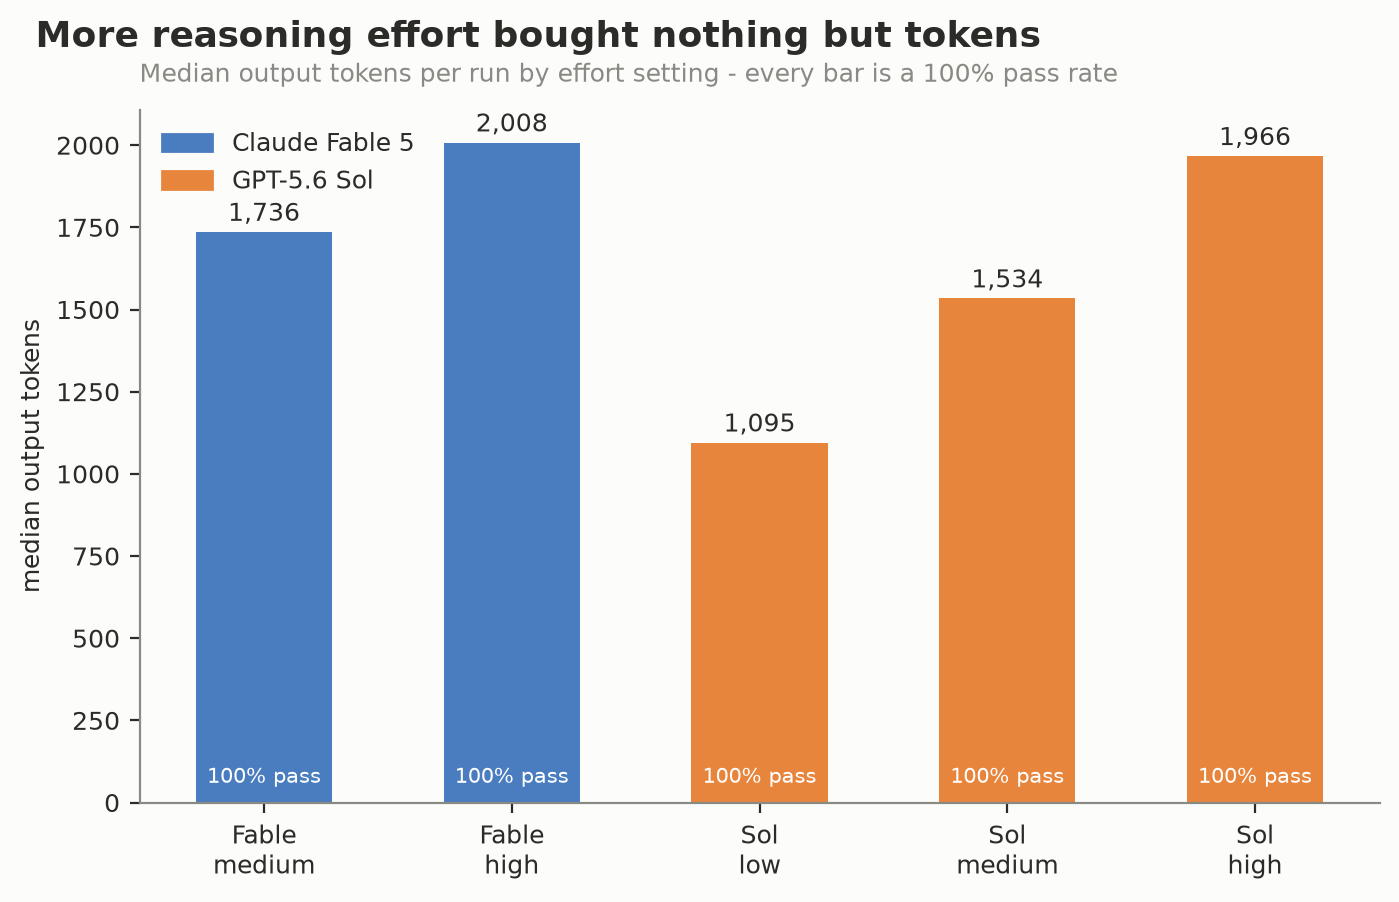
\includegraphics[width=0.9\linewidth]{2-effort-buys-nothing.png}
\caption{Output tokens by effort level. Tokens climb with the effort
setting; every marker is a 100\% pass. Effort buys tokens, not outcomes.}
\label{fig:effort}
\end{figure}

\subsection{Different animals, same destination}

The models' solution styles differ sharply. \fable{} iterates: median 6--7
turns per task, $\approx$59--68\,s wall clock --- read, edit, check, edit
again. \sol{} one-shots: median 1 turn, $\approx$26--64\,s --- internal
reasoning, then a single emitted solution. Neither style won on outcomes,
because both cleared the tier. Turn count is a workflow signature, not a
quality signal.

\subsection{The harness did not move pass rate}

Paired bare-vs-harnessed comparisons at each model's winning effort (14
pairs each) again produced zero discordant pairs: $100\% \to 100\%$. The
harness was designed for longer, messier work than these tasks; on this
suite it changed token spend (Fable $-560$ mean tokens; Sol $+71{,}624$,
driven by its instruction-context handling) but not outcomes.

\subsection{Token economics: who is cheaper per solved task?}
\label{sec:inputtokens}

Table~\ref{tab:perm} reports the exact sign-flip permutation test
(Eq.~\ref{eq:permutation}) on per-task median $\log$(total tokens) over
passing runs. All nine paired differences favor \fable{}; the observed sum
of differences is $-17.72$, and 2 of $2^9 = 512$ sign patterns are as or
more extreme, giving two-sided $p = 0.0039$. By its own CLI's accounting,
\fable{} is roughly $6$--$10\times$ cheaper in total tokens per solved task
on this suite.

\begin{table}[H]
\centering
\small
\begin{tabular}{lccc}
\toprule
task & Fable med $\log(\text{tok})$ & Sol med $\log(\text{tok})$ & diff (F$-$S) \\
\midrule
t1-py-a & 9.9293  & 11.7945 & $-1.8652$ \\
t1-py-b & 9.9256  & 11.7996 & $-1.8739$ \\
t1-ts-a & 9.9218  & 11.7104 & $-1.7886$ \\
t1-ts-b & 9.9579  & 11.9564 & $-1.9985$ \\
t2-py-a & 9.9333  & 11.6615 & $-1.7282$ \\
t2-py-b & 9.9590  & 12.0185 & $-2.0595$ \\
t2-ts-a & 10.0253 & 12.2987 & $-2.2734$ \\
t2-ts-b & 9.9256  & 11.9755 & $-2.0499$ \\
t3-a    & 9.8712  & 11.9511 & $-2.0799$ \\
\midrule
\multicolumn{3}{l}{sum of diffs $=-17.7172$; \; 2 of 512 patterns as-or-more extreme}
& $p = 0.0039$ \\
\bottomrule
\end{tabular}
\caption{Exact sign-flip permutation test on per-task median
$\log$(total tokens) over passing runs, paired by task.}
\label{tab:perm}
\end{table}

\paragraph{A caveat you cannot skip: input tokens do not compare across
vendors.} \fable{}'s CLI reports $\approx$19.4k median input tokens; \sol{}'s
reports 95k--175k. That is not \sol{} reading $5$--$9\times$ more code: the
two CLIs count context resends and cache reads differently, so their
input-token numbers measure different things under the same label
(Figure~\ref{fig:input}). Within-model comparisons are safe (each CLI is
self-consistent); cross-model input-token or dollar comparisons are
indicative only, and we do not publish them as hard claims. The honestly
cross-comparable axes are output tokens, turns, and wall-clock time.

\begin{figure}[H]
\centering
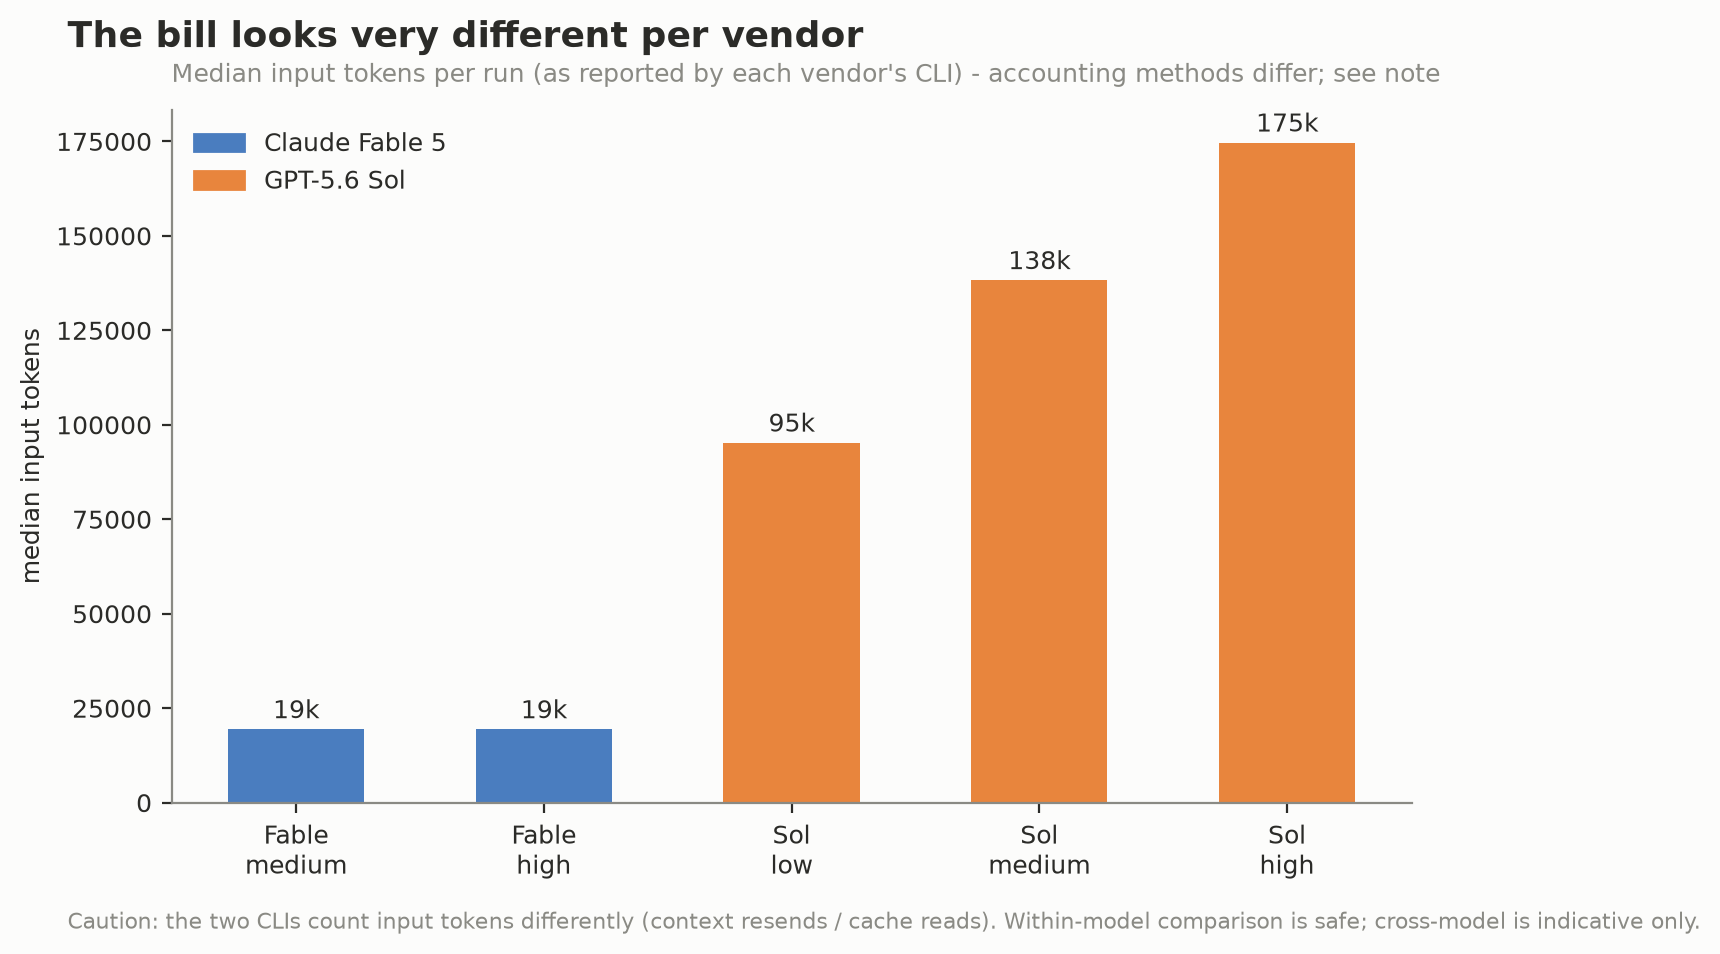
\includegraphics[width=0.9\linewidth]{3-input-token-economics.png}
\caption{Input tokens by configuration. The cross-model gap is an artifact
of CLI bookkeeping, not workload; the chart carries the caveat on its face.}
\label{fig:input}
\end{figure}

\subsection{The hybrid arm: full disclosure}
\label{sec:hybrid}

We also tested a hybrid configuration --- \fable{} orchestrating \sol{} as
the implementer --- on the greenfield task. It was the only configuration
that did not run clean. Across four attempts, two produced planning notes
and zero code; two shipped working solutions of $\approx$160--176 lines:
\textbf{2 of 4}. The official results file records the two later, successful
attempts; the two earlier failures are disclosed here. The rig was identical
across all four attempts, so the most defensible reading is genuine
run-to-run variance in a multi-agent handoff, not a fixed defect --- and at
$n=4$ we decline to build any stronger story. It is a flag for the next
experiment, not a conclusion.

\subsection{Judge agreement}
\label{sec:judges}

Across 139 dual-judged runs (each judge's score averaged over its four
rubric axes): mean absolute gap \textbf{0.53} points on a 0--10 scale,
Pearson $r = 0.76$, and \textbf{96\%} of runs within $\pm 1$ point. On the
pilot, the GPT judge scored $\approx$0.5 points more generous than the
Claude judge on the same diffs, and both judges leaned slightly toward
\sol{}'s code --- precisely the self-preference risk that motivated blind,
dual judging~\cite{wataoka2024selfpreference}, and precisely why we report
the disagreement instead of averaging it away.

% ---------------------------------------------------------------- section 6
\section{Limitations}

This section is the credibility of the study; we state each limit bluntly.

\begin{enumerate}
  \item \textbf{Small per-arm samples.} At $n=24$ per arm the design has
        80\% power only for gaps $\gtrsim 36.7$ percentage points at a 50\%
        baseline (Eq.~\ref{eq:power}). Smaller real differences get a
        confidence interval, not a verdict.
  \item \textbf{Ceiling effect.} Because both models passed everything, the
        suite cannot \emph{rank} them --- it only establishes that both
        clear this tier. Reading ``154 perfect runs'' as ``the models are
        identical'' over-reads the data.
  \item \textbf{Model judges, not humans.} Blind, dual, disagreement
        reported --- but still automated graders with their own biases.
  \item \textbf{One re-run.} A single \fable{} greenfield run hit a
        transient CLI error (2.3\,s, zero tokens) and was re-run. Disclosed.
  \item \textbf{AI-assisted task authoring.} Tasks were proven solvable, but
        their difficulty was mis-calibrated low. That miscalibration is not
        a footnote; it \emph{is} the headline finding.
  \item \textbf{No dollar claims.} Cost figures use list-price placeholders
        over vendor-incomparable token counts and are not published as
        dollar claims.
  \item \textbf{Long-context (``dumb zone'') asymmetry.} Practitioner
        experience and published long-context research find that model
        quality degrades as context grows large ($\sim$100k
        tokens)~\cite{liu2024lost}. By its own CLI's accounting, \sol{}
        exceeded 100k cumulative input tokens on 65 of its 88 runs (median
        142k, max 353k); \fable{} peaked at 19.6k. Two qualifiers: the
        \texttt{codex} CLI counts context resends across internal steps, so
        live context occupancy at any moment is not observable from our
        data; and the bias runs \emph{against} \sol{}, which passed
        everything anyway. The tie is therefore safe, but blind-judge
        quality comparisons carry this asymmetry, and it is on the record.
\end{enumerate}

% ---------------------------------------------------------------- section 7
\section{Future work}

A ceiling tells you exactly where to point the next experiment. Experiment~2
is a hard tier (T4): the same rig, blocking, blind dual judging, and exact
statistics, with task difficulty raised until failures appear. Failures are
the requirement --- a gap becomes measurable only once at least one model
starts missing, and the effort dial can only earn its cost once ``think
harder'' changes an outcome rather than a token count. Same exam room,
harder exam.

\section*{Acknowledgments}
The experiment harness, task suite, dual-judge pipeline, and statistical
appendix are maintained in a private repository; the statistical
methodology is grounded in the author's industrial-engineering coursework
(Georgia Tech ISyE): hypothesis testing, confidence intervals, design of
experiments, and stochastic processes.

% ---------------------------------------------------------------- appendix
\appendix
\section{Reproducibility}
\label{app:repro}

Every number in this report is produced by a dependency-free script from the
raw logs:

\begin{quote}
\ttfamily
python3 runner/stats.py -{}-results runner/results/results.jsonl \\
\hspace*{2em} -{}-judgments runner/results/judgments.jsonl
\end{quote}

The script emits the statistical appendix (per-cell Wilson CIs, every
McNemar $2\times2$ table with its exact $p$-value, the token permutation
test, judge agreement, and the power statement) and carries a self-test mode
(\texttt{-{}-selftest}) checking the primitives against known values:
McNemar exact $p(b{=}1, c{=}5) = 0.21875$; Wilson 95\% CI for $8/10 =
(0.4901,\,0.9433)$; sign-flip $p$ for eight positive differences $= 2/256 =
0.0078125$; Pearson $r = 1.0$ on exact linear data. All checks pass.

Judging is blind and dual: transcripts and diffs are stripped of identity
before either judge scores them, and both a Claude judge and a GPT judge
score every run on the same four-dimension rubric.

% -------------------------------------------------------------- references
\begin{thebibliography}{9}\small

\bibitem{jain2024livecodebench}
N.~Jain, K.~Han, A.~Gu, W.-D.~Li, F.~Yan, T.~Zhang, S.~Wang, A.~Solar-Lezama,
K.~Sen, and I.~Stoica.
\newblock LiveCodeBench: Holistic and contamination free evaluation of large
language models for code.
\newblock \emph{arXiv:2403.07974}, 2024.

\bibitem{sui2025overthinking}
Y.~Sui et al.
\newblock Stop overthinking: A survey on efficient reasoning for large
language models.
\newblock \emph{arXiv:2503.16419}, 2025.

\bibitem{su2025underthinking}
A.~Su et al.
\newblock Between underthinking and overthinking: An empirical study of
reasoning length and correctness in LLMs.
\newblock \emph{arXiv:2505.00127}, 2025.

\bibitem{wataoka2024selfpreference}
K.~Wataoka, T.~Takahashi, and R.~Ri.
\newblock Self-preference bias in LLM-as-a-judge.
\newblock \emph{arXiv:2410.21819}, 2024.

\bibitem{liu2024lost}
N.~F.~Liu, K.~Lin, J.~Hewitt, A.~Paranjape, M.~Bevilacqua, F.~Petroni, and
P.~Liang.
\newblock Lost in the middle: How language models use long contexts.
\newblock \emph{Transactions of the Association for Computational
Linguistics}, 12:157--173, 2024. arXiv:2307.03172.

\bibitem{wilson1927}
E.~B.~Wilson.
\newblock Probable inference, the law of succession, and statistical
inference.
\newblock \emph{Journal of the American Statistical Association},
22(158):209--212, 1927.

\bibitem{mcnemar1947}
Q.~McNemar.
\newblock Note on the sampling error of the difference between correlated
proportions or percentages.
\newblock \emph{Psychometrika}, 12(2):153--157, 1947.

\bibitem{fisher1935}
R.~A.~Fisher.
\newblock \emph{The Design of Experiments}.
\newblock Oliver and Boyd, Edinburgh, 1935.

\bibitem{montgomery2017doe}
D.~C.~Montgomery.
\newblock \emph{Design and Analysis of Experiments}.
\newblock Wiley, 9th edition, 2017.

\end{thebibliography}

\end{document}
